\documentclass[final]{fhnwreport}         %[mode] = draft or final
\input{fhnwheader}                        %loads all packages, definitions and settings

%%%%% Logo: Hochschule HTU oder HSI, Sprache DE oder EN:
%\newcommand{\logofilename}{FHNW_HTU_DE}
%\newcommand{\logofilename}{FHNW_HTU_EN}
%\newcommand{\logofilename}{FHNW_HSI_DE}
\newcommand{\logofilename}{FHNW_HSI_EN}
%%%%%
%%%%% Bibliographie entweder im IEEE- oder im APA-Stil:
\usepackage[style=ieee,urldate=comp,backend=biber]{biblatex}
%\usepackage[style=apa,urldate=comp,backend=biber]{biblatex}
%%%%%
\addbibresource{literature/references.bib}

\title{IP6: Troubleshooting Network Problems With An AI Driven Multi-Agent System}  %Project Title
\author{P6 Project}    %Document Type => Technical Report, ...
\date{Windisch, \today}               %Place and Date

\begin{document}

\pagenumbering{roman}

%%---TITLEPAGE---------------------------------------------------------------------------
\selectlanguage{english}                  %ngerman or english
\maketitle

\vfill

\begin{tabular}{@{}p{5cm} l}
Student          &    Dominik Krebs\\[2ex]
Experts           &    Christopher Scherb / Luc Heitz\\[2ex]
Project Number              &    IMVS12\\[4ex]
\multicolumn{2}{@{}l}{University of Applied Sciences Northwestern Switzerland}
\end{tabular}

\clearpage

%%---ABSTRACT----------------------------------------------------------------------------
\selectlanguage{english}				%ngerman or english
\thispagestyle{empty}
\section*{Abstract}

Troubleshooting computer networks is a complex, mostly manual activity. A network operator
works from the first symptom through device after device until a root cause is found. This
project investigates whether an AI-driven multi-agent system can take over this troubleshooting work
and at what benefit and cost. A system was built in which an orchestrator agent splits a
troubleshooting request and delegates the tasks to specialised agents, all operating against live network devices.

The system was evaluated in a containerlab environment of Nokia SR Linux devices using ten reproducible 
scenarios (a healthy baseline plus nine injected faults across three
difficulty tiers) and six language models from three price tiers. Each of the 300 runs
(10 scenarios $\times$ 6 models $\times$ 5 repetitions) was evaluated manually against the
scenario's known root cause.

The results show that the outcome depends mainly on the model used. With identical
agent logic, the success rate spans 16\,\% to 100\,\%. The high-tier models diagnosed 98 of 100
runs correctly across all difficulty tiers. They were typically within about two to three minutes and almost
independently of fault difficulty. Mid-tier models were reliable on easy faults (74--82\,\%
overall) but failed on harder faults, mostly
by hitting the time cap rather than by giving a wrong result. Low-tier models were
unusable and one of them repeatedly invented faults in a healthy network. With the mid- and high-tier
models, a correct diagnosis cost \$0.21--\$2.91 in API fees, a fraction of the
network operator time it replaces. Within the limits of a small single-fault lab, the experiments
show that autonomous multi-agent network troubleshooting works today when a sufficiently capable
model is used.

\vspace{2ex}


%%---TABLE OF CONTENTS-------------------------------------------------------------------
\selectlanguage{english}				%ngerman or english
\tableofcontents
\clearpage

\listoffigures
\listoftables
\cleardoublepage

%%---TEXT--------------------------------------------------------------------------------
\pagenumbering{arabic}
\section{Introduction}
\label{sec:introduction}

Troubleshooting computer networks is a time-consuming and still largely manual
activity. When a service reports a problem or a host loses connectivity, an
engineer needs to consult the available tools and check one device after another, running
show commands, inspecting interface counters, routing tables, ARP caches
and syslog messages until a fault is localised. The path from the first symptom to the true root cause
often requires a lot of steps and time. As networks
grow in size and complexity, this diagnostic effort translates directly into
operational cost and into mean-time-to-repair.

Recent advances in large language models (LLMs) and, in particular, in
agentic systems that let an LLM call external tools, observe the results
and decide on the next action, suggest a new way to support this work. Instead of
a single agent model, a multi-agent system can decompose the problem
into smaller parts and assign them to specialised agents. 
Whether such a system can be used to assist in troubleshooting or even find problems autonomously is an open
and practically relevant question.

\subsection{Project goal}

The goal of this project is to design and build an AI-driven multi-agent system
for network troubleshooting and to use it as an instrument to evaluate
\emph{which kinds of network problems can realistically be troubleshooted by such
a system, and at what benefit and cost}. 

\subsection{Research questions}
\label{sec:research-questions}

The project is guided by four research questions:

\begin{enumerate}
  \item \textbf{Time}: How much time can be saved in troubleshooting by using the
        agent network compared to a manual workflow?
  \item \textbf{Difficulty}: Problems of which difficulty level can be
        troubleshooted by the agent network?
  \item \textbf{Success rate}: What is the success rate for the correct analysis
        of the problems at each difficulty level?
  \item \textbf{Cost}: How much can potentially be saved or, conversely, how
        much does it cost to use an agent network for troubleshooting network
        issues, and how does this depend on the chosen model?
\end{enumerate}


\subsection{Outline}

\Cref{sec:background} introduces the underlying technologies. LLMs, AI agents,
function calling, the agent loop and the Model Context Protocol.
\Cref{sec:concepts} explains how these building blocks are combined into the
multi-agent troubleshooting system and \cref{sec:implementation} describes its
realisation. \Cref{sec:methodology} defines the fault scenarios, the
difficulty tiers, the evaluated models and the experiment procedure.
\Cref{sec:results} reports the measurements, \cref{sec:evaluation} interprets
them with respect to the research questions and discusses the limitations, and
\cref{sec:conclusion} concludes the report and outlines future work.
\section{Background}
\label{sec:background}
This section gives the necessary background information about the technologies used in this work to build an AI agent.

\subsection{Agents and AI Agents}
// TODO

\subsubsection{Agent}
From a very basic perspective, an agent is an entity which is able to produce some effect or make changes in its
environment \parencite{CASTELFRANCHI1998157}.

\subsubsection{AI Agent}
\label{sec:AI_Agent}
With the rise of generative AI a new term "AI Agent" has emerged.
AI Agents can be defined as software entities which are designed to fulfill goal-oriented tasks.
Such agents can take in information from their environment, be it structured or unstructured inputs, draw conclusions from
the context and initiate actions toward achieving specific objectives. Rather than executing a
predetermined and deterministic sequence of steps like a traditional agent, an AI Agent can respond to what it observes while running,
adjusting its behaviour and the results it produces as the situation changes. The primary decision-making engine for these
AI Agents are LLMs (see \cref{sec:LLMs}) \parencite{Sapkota_2026}.



\subsection{Large Language Models (LLMs)}
\label{sec:LLMs}
Large Language Models (LLMs) are an evolution
 in artificial intelligence, moving from
 rule-based systems to general-purpose generative models. An LLM is essentially
 a complex statistical system designed to predict the likelihood of
 a sequence of words. By training on massive amounts of text, often
 using lots of data from the public internet. These
 models learn to generate coherent and contextually appropriate
 continuations for a given input prompt \parencite{douglas2023largelanguagemodels}.


\subsection{Tokens, Context Windows and Cost}
\label{sec:tokens-context-cost}
LLMs do not operate on text (words and characters) directly. Text has to first go through a \emph{tokenizer} that breaks it into pieces called \emph{tokens}
which can be words, sub-words or even just single characters. The goal of a \emph{tokenizer} is to return an efficient set of tokens to represent a text dataset. \parencite{alammar2024hands}

Each model can only process a limited number of tokens at once. This upper bound is referred to as the
\emph{context window} and covers the prompt, any provided tools, the conversation history and the generated
response. Beyond being a hard limit, longer contexts also degrade the quality of the model's output:
\textcite{liu-etal-2024-lost} show that models use information most reliably when it appears at the beginning or the
end of the context and perform noticeably worse when relevant information is located in the middle, a
phenomenon known as "lost in the middle". The degradation is not only a question of \emph{where} relevant
information sits, but also of \emph{how much} context surrounds it: \textcite{hong2025context} evaluate a
range of state-of-the-art models on deliberately simple tasks and find that performance declines, as the input grows longer, even when the task itself does not become harder. These two properties, the finite context window and the
degradation over long contexts, are a central motivation for distributing work across several specialised
agents rather than handling everything in a single, ever-growing context (see \cref{sec:multi-agent}).


\subsection{Multi-Agent (AI) Systems}
\label{sec:multi-agent}
A multi-agent (AI) systems (MAS) are systems composed of multiple interacting agents. 
MAS (Multi-agent systems) are able to solve more difficult problems compared to individual agents (a monolithic system) \parencite{tran2025multiagentcollaborationmechanismssurvey} 

With the rise of LLM-based agents (AI Agents) (see \cref{sec:LLMs}), this idea has been transferred to systems in which
the individual agents are driven by LLMs. \textcite{tran2025multiagentcollaborationmechanismssurvey} work describes how
multiple LLM agents collaborate through different coordination structures. This work uses a \emph{hierarchical} structure together with
a \emph{role-based} collaboration strategy. A detailed view of the architecture in this work is described in \cref{sec:concepts}.

Splitting a task across several specialised agents has practical benefits that follow directly from the
limitations discussed in \cref{sec:tokens-context-cost}: each agent can be given a focused instruction set and
a smaller selection of tools, which keeps its individual context small, reduces the risk of context-related
quality degradation.




\subsection{Function Calling}
\label{sec:func-calling}
LLMs have great generative capabilities but they lack the ability to perform any task beyond generating a response.
This means LLMs are not able to retrieve any external information in real time. 
This limitation means LLMs only have access to the static training data, this inherently results in reponses that are plausible but factually incorrect or outdated (often referred to
as hallucination). \parencite{Qu_2025}. 
To address this limitation a paradigm named "Function Calling" has been developed. 
It solves these problems by giving LLMs the ability to interact with external systems by invoking predefined blocks of code (functions) \parencite{wang2026FunctionCalling}.

\subsubsection{Function Calling process example using OpenAI API}
The following Image illustrates the function calling principle using the OpenAI function calling API as an example. The function calling API is an optional part of the new \emph{Responses API} or the older \emph{Chat Completions API} \parencite{openai_responses_create}.

\begin{enumerate}
    \setlength{\itemsep}{8pt}
    \item The prompt message and all the tool definitions are sent to the model.
    \item Based on the provided prompt and tools the model decides to call some function, providing the necessary arguments (in this example "paris").
    \item The function chosen by the model is executed.
    \item All prior messages together with the result (output) of the function execution are sent back to the model.
    \item Based on all the messages the model gives back a final response \parencite{openai_function_calling}.
\end{enumerate}

\begin{figure}[htbp]
\begin{center}
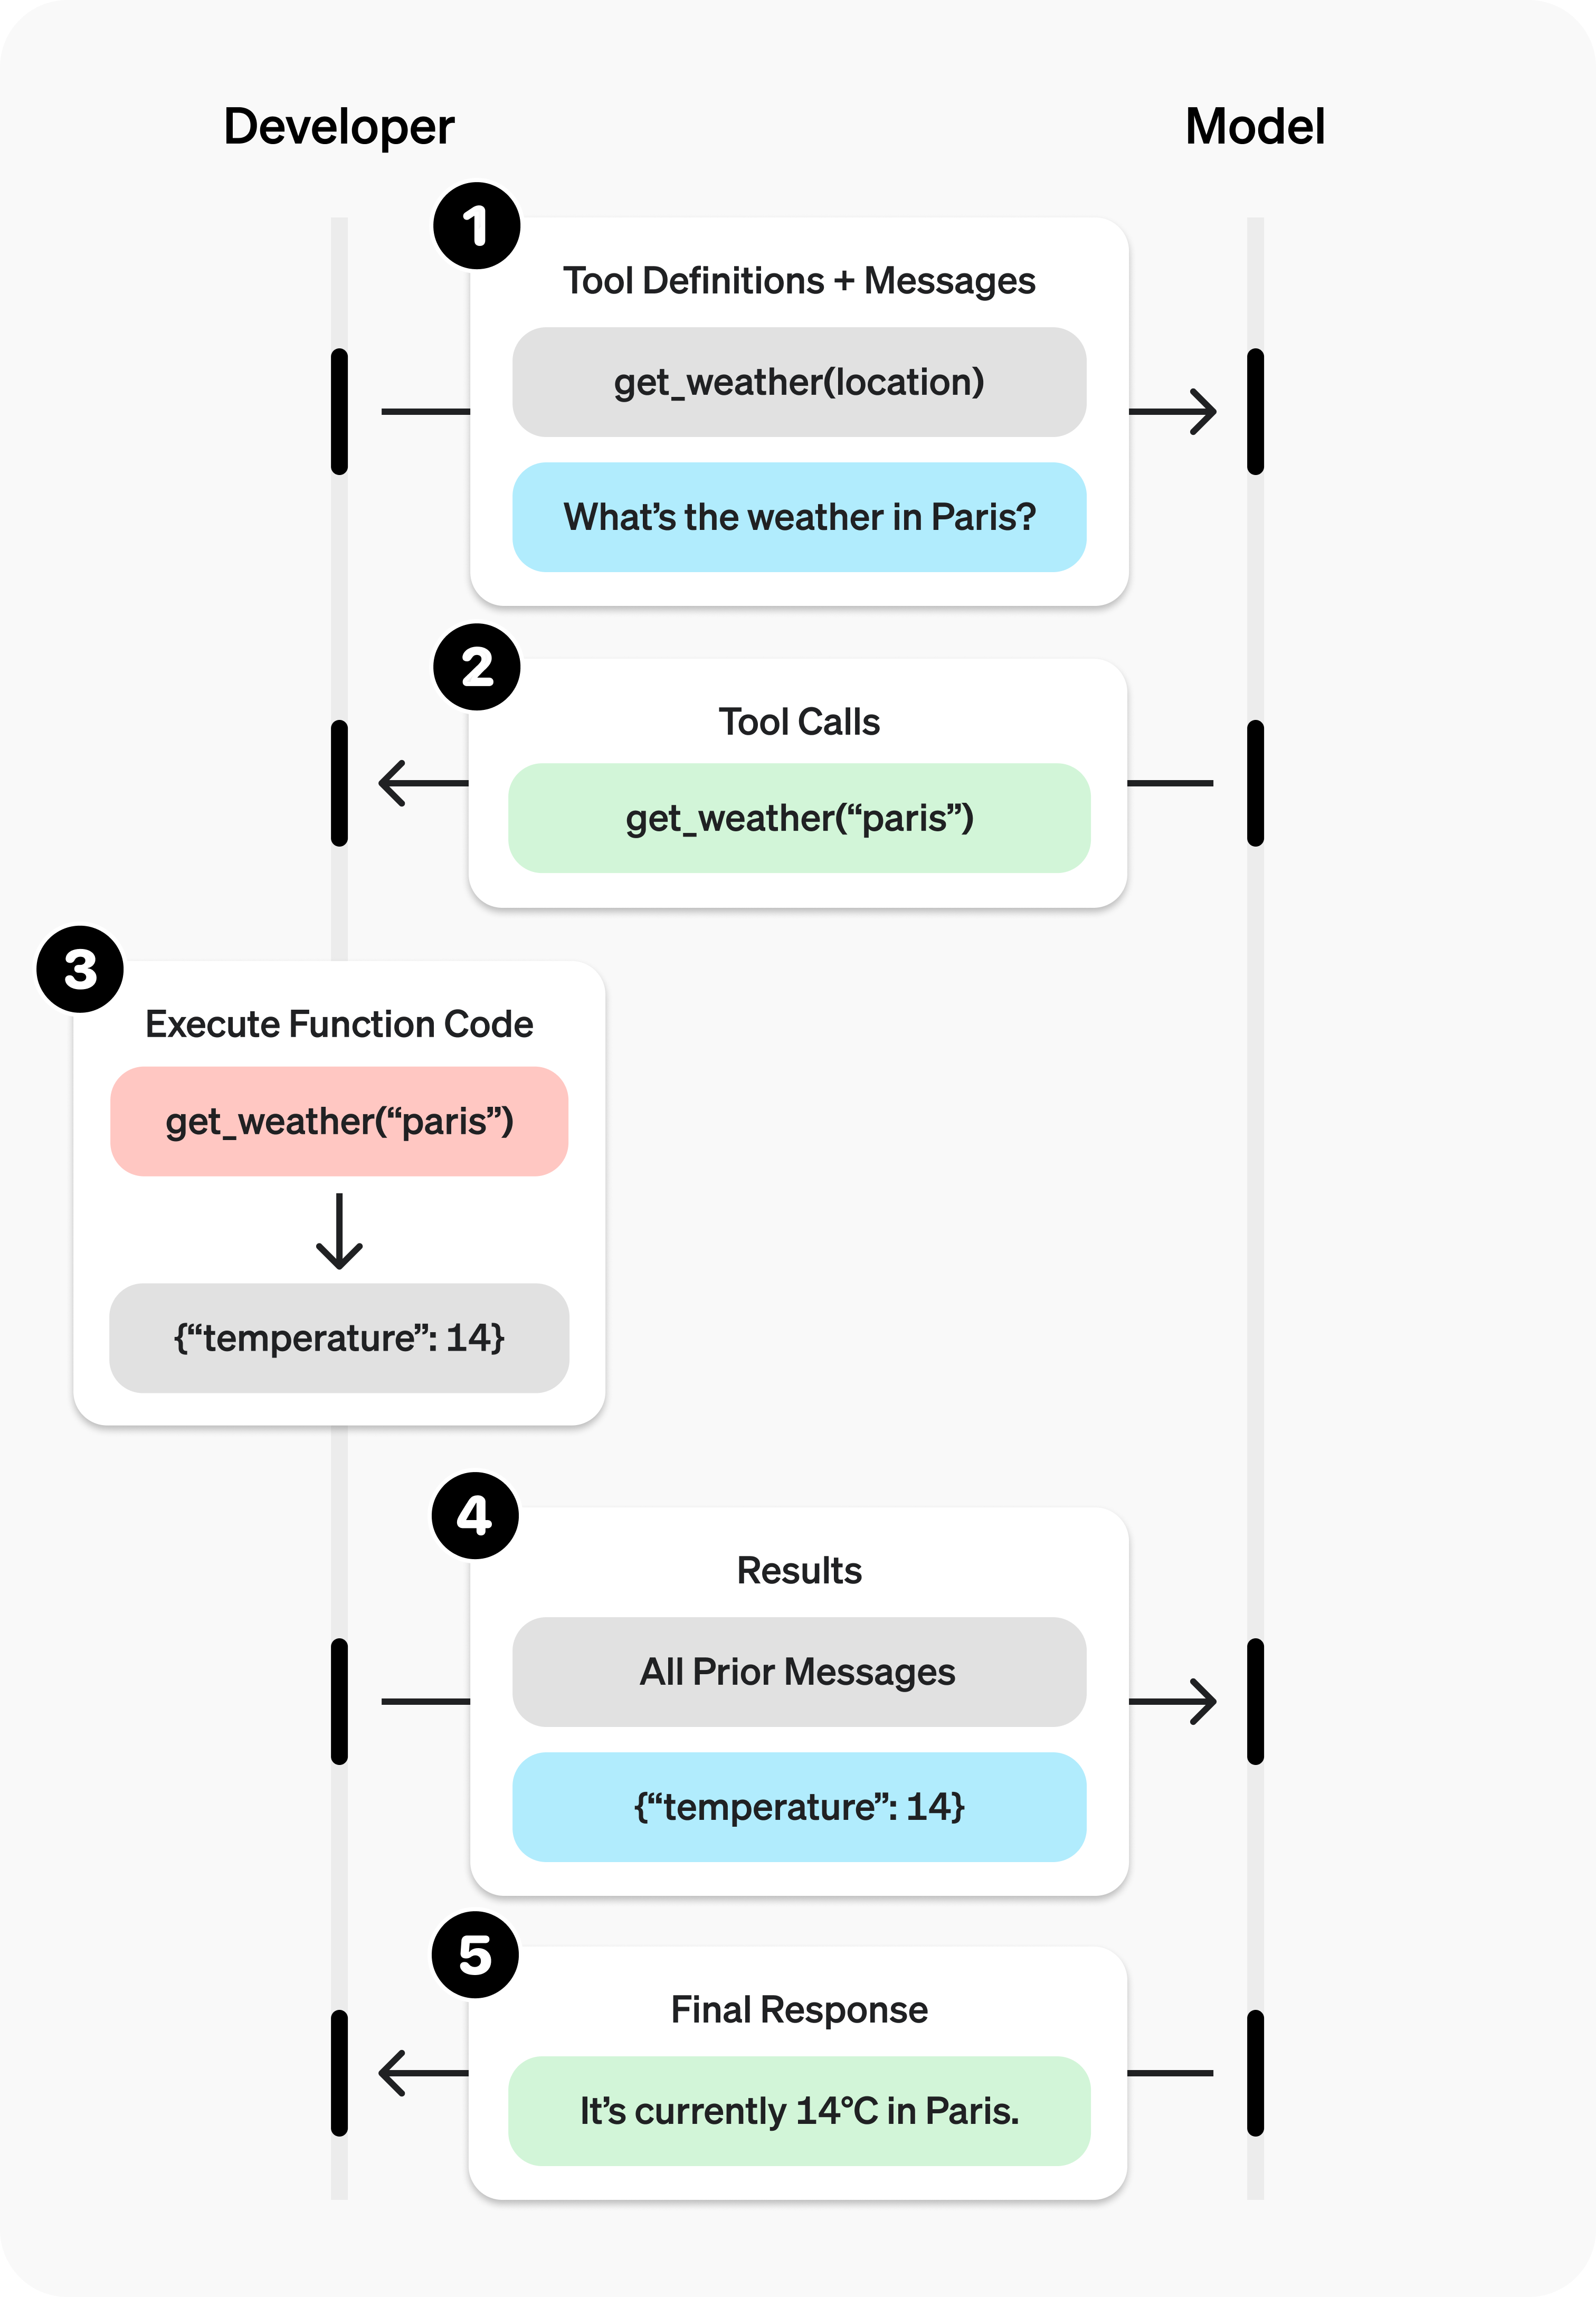
\includegraphics[width=0.9\linewidth]{graphics/function-calling-diagram-steps.png}
\end{center}
\caption{Function calling procedure
\parencite{openai_function_calling}}
\label{fig:function-calling-procedure}
\end{figure}

\newpage
\subsection{Agent Loop and Agent Harness}
\label{sec:agent-loop}

\subsubsection{Agent Loop}
Function calling (see \cref{sec:func-calling}) describes a \emph{single} exchange in which the model receives a function, requests a
function execution and receives its result. On its own, this does not yet make a system agentic. The model still needs to be
invoked repeatedly, decide when another tool call is necessary, and recognise when the task is complete. This
repetition is captured by the term \emph{agent loop}, the core control cycle of an AI Agent. The model receives the current
context, decides on an action (either calling a tool or producing a final answer), the chosen tool is executed, its
result is appended to the context, and the cycle repeats until the model returns a final answer or a stop condition is
reached \parencite{yao2023reactsynergizingreasoningacting,anthropic_effective_agents,strands_agent_loop}. These steps of reasoning and acting were introduced
as the \emph{ReAct} pattern by \textcite{yao2023reactsynergizingreasoningacting}. The agent loop is therefore what elevates a sequence of isolated
function calls into goal-oriented behaviour that adapts to what the model observes while running, as introduced in
\cref{sec:AI_Agent}.

\Cref{fig:agent-loop} shows this cycle: an initial input and context enter the loop, the model reasons and selects a
tool, the tool is executed and its result is fed back for the next round of reasoning, and the loop repeats until the
model produces a final response.

\begin{figure}[htbp]
\begin{center}
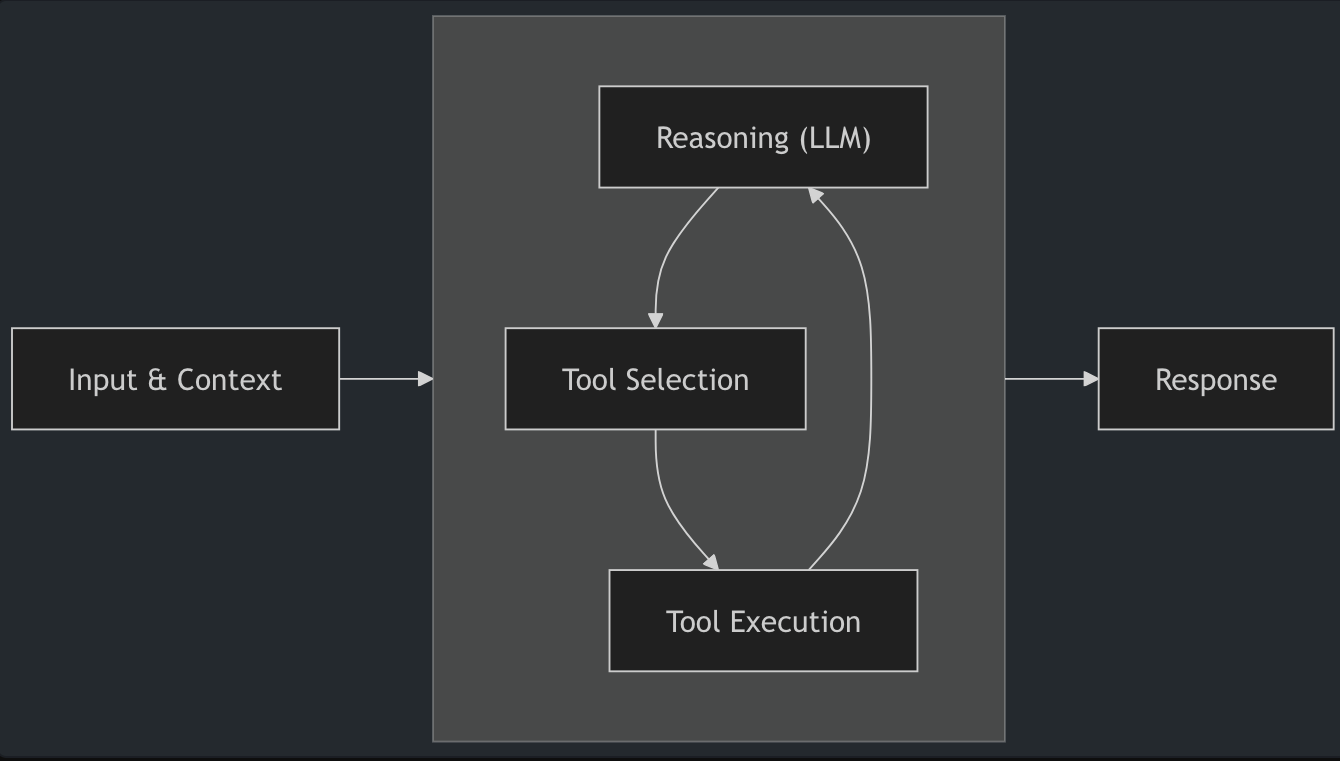
\includegraphics[width=0.9\linewidth]{graphics/agent-loop-strandsagents.png}
\end{center}
\caption{The agent loop \parencite{strands_agent_loop}}
\label{fig:agent-loop}
\end{figure}
\newpage

\subsubsection{Agent Harness}
An LLM by itself cannot run this loop (agent loop), it only predicts a single continuation for a given input
(see \cref{sec:func-calling}). The loop, the dispatching of tool calls, the accumulation of the message history and the
evaluation of stop conditions all have to be implemented by the surrounding software. This runtime software is
commonly referred to as the \emph{agent harness}, the software infrastructure that wraps around an LLM and enables it to
act on tasks rather than only respond to prompts, often summarised as \emph{Agent = Model + Harness}
\parencite{databricks_ai_harness,langchain_agent_harness}. The harness is the engine that drives the agent loop (the core) and manages the
things around it. It forwards the conversation and the available tool definitions to the model, executes the tool
calls the model requests and maintains the message history across iterations. In practice a
harness is most of the time provided by an \emph{agent framework} with APIs to modify and add additoanl functionalities. The concrete framework used in this work is described in
\cref{sec:implementation}.

\Cref{fig:agent-harness} illustrates this relationship: the model sits at the centre and only reasons and decides,
while everything around it, the context injection, control, action (tool calls), observation and persistence, is
provided by the surrounding harness.

\begin{figure}[htbp]
\begin{center}
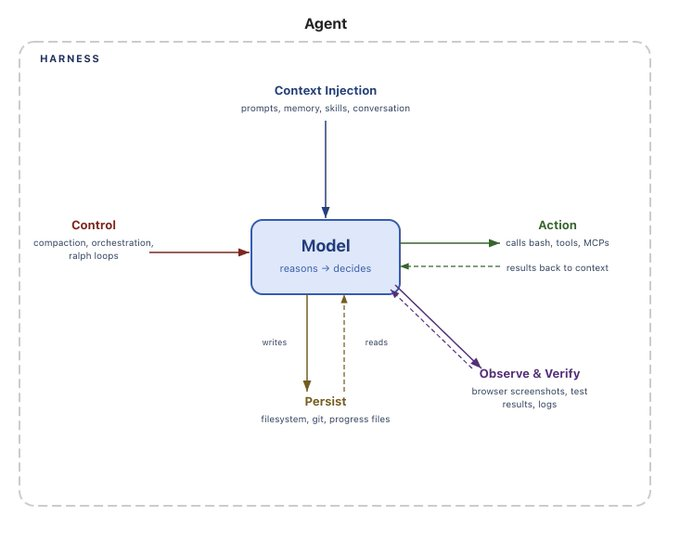
\includegraphics[width=0.9\linewidth]{graphics/langchain-anatomy-of-an-agent-harness.png}
\end{center}
\caption{Anatomy of an agent: the model surrounded by the harness
\parencite{langchain_agent_harness}}
\label{fig:agent-harness}
\end{figure}


\newpage
\subsection{Model Context Protocol (MCP)}
\label{sec:mcp}
The Model Context Protocol (MCP) is an open-source standard designed to facilitate the connection between AI
 applications and external systems. MCP allows AI models (such as ChatGPT) to securely interact with different
 data sources (like local files and databases) and tools (execute functions).

The core problem MCP addresses is the fragmentation of AI integrations. Before MCP, every
new data source required its own custom implementation, making truly connected systems
difficult to scale \parencite{mcp_anthropic}. This is commonly framed as the $N \times M$
integration problem \parencite{mcp_nxm}. Without a common standard, connecting $N$ AI
applications to $M$ external systems (data sources and tools) requires a custom 
integration for every AI-Application, external system pair, resulting in up to $N \times M$ separate
integrations that must each be built and maintained individually. MCP replaces this with a
single shared protocol. Every AI application implements the MCP client side once, and every
external system is exposed through an MCP server once. This reduces the integration effort
from a multiplicative $N \times M$ to an additive $N + M$. 
\parencite{mcp_nxm}.

As illustrated in \cref{fig:mcp_architecture-overview}, MCP therefore functions similarly to a
"USB-C port for AI applications," providing a standardized way to connect AI
applications to external systems \parencite{mcp_intro}.

\begin{figure}[htbp]
\begin{center}
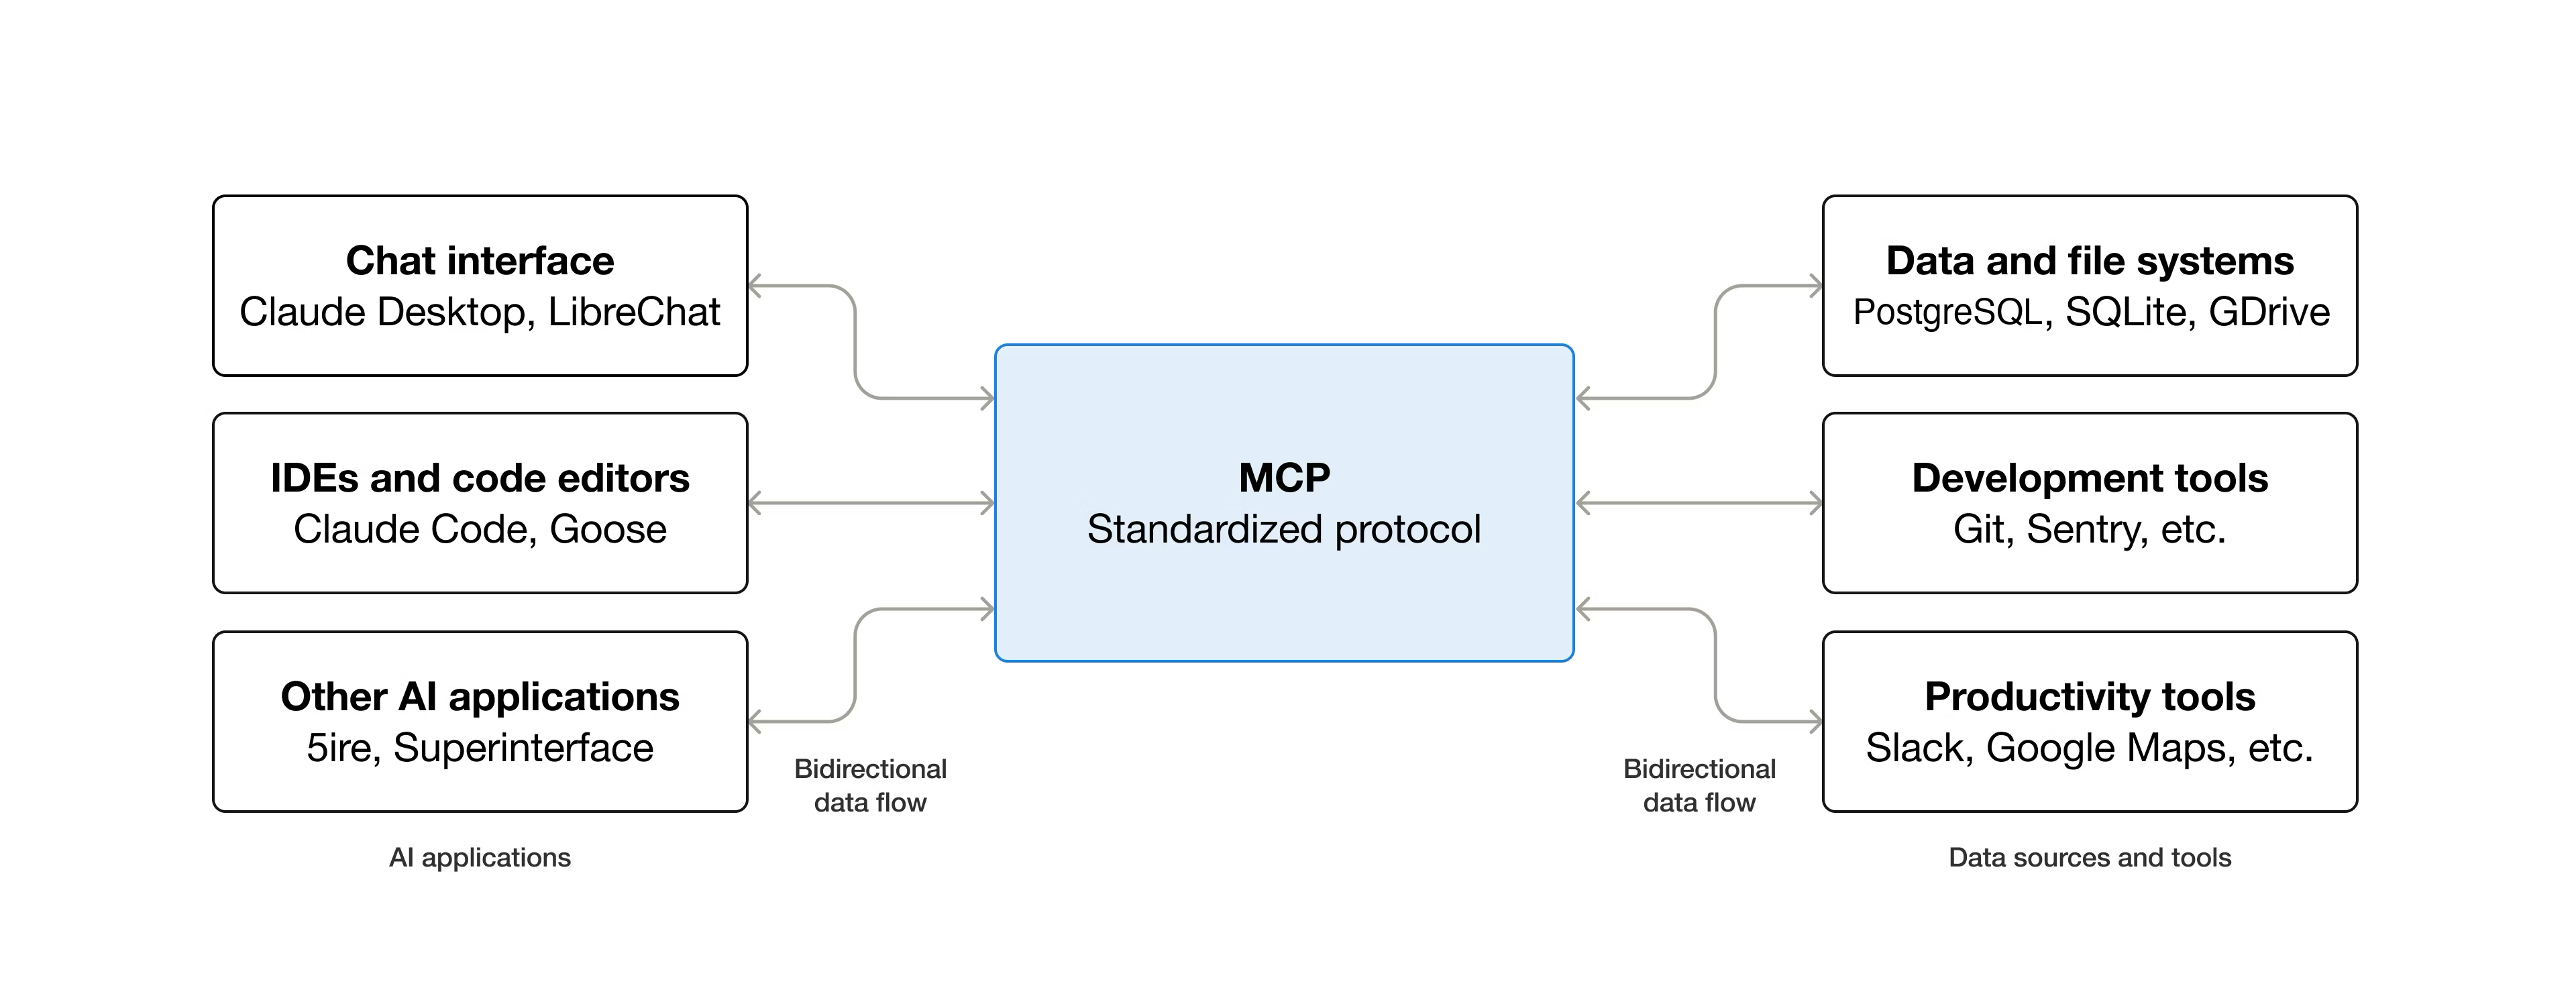
\includegraphics[width=0.9\linewidth]{graphics/mcp-architecture-overview.png}
\end{center}
\caption{MCP architecture
\parencite{mcp_intro}}
\label{fig:mcp_architecture-overview}
\end{figure}







\section{Concepts}
\label{sec:concepts}
This section describes the conceptual design of the multi-agent troubleshooting system. While
\cref{sec:background} introduced the underlying technologies in general terms, this section explains
\emph{how} these concepts are applied to the problem of network troubleshooting and, more importantly,
\emph{why} the system is designed the way it is. The realisation (implementation) in code is deferred to
\cref{sec:implementation}, and the experimental procedure used to evaluate the design is described in
\cref{sec:methodology}.


\subsection{Scope: Two Independent Parts}
\label{sec:concepts-scope}
The work described in this report consists of two distinct and largely independent parts, which it is
important to keep apart conceptually.

The \emph{first part} is the core of the project and addresses the research questions stated in
\cref{sec:introduction}: which network problems can be troubleshooted by a multi-agent system, with what
success rate across difficulty levels, and at what cost. This part is driven by a human operator who poses a
troubleshooting goal to the user-facing orchestrator, and it is evaluated quantitatively against a catalogue
of reproducible fault scenarios (see \cref{sec:evaluation-concept,sec:model-tier-concept}). The bulk of the
architecture, the agent roles and the evaluation concept described below serve this first part.

The \emph{second part} is an independent feasibility use case rather than a measured research question: the
\emph{automatic syslog investigation}. The motivating question here is not \emph{how well} or \emph{at what
cost}, but simply \emph{whether} it is possible to build a system that reacts autonomously to certain syslog
messages and starts a self-contained initial investigation without any human trigger. How such a mechanism works in
practice and how a human operator can take over and continue the troubleshooting without
repeating the work the autonomous investigation has already done. This use case reuses the same
agents shown and described in \cref{fig:architecture-overview} building blocks but it uses a different entry point (\texttt{investigation\_orchestrator}). It is described on its own in
\cref{sec:autonomous-syslog-usecase} and is not part of the quantitative evaluation.

\subsection{Overall Architecture}
\label{sec:architecture}
The system is structured as a \emph{hierarchical}, \emph{role-based} multi-agent system, the collaboration
pattern introduced in \cref{sec:multi-agent}. A central \emph{orchestrator} agent receives a troubleshooting
goal and delegates focused sub-tasks to a set of specialised sub-agents, each responsible for one domain of
the network (see \cref{sec:agent-roles}).

The decisive reason for distributing the work across several agents rather than handling it in a single,
monolithic agent follows directly from the limitations discussed in \cref{sec:tokens-context-cost}. A single
agent would have to hold the entire troubleshooting context (all tool definitions, all device output, the full
conversation history) in one large context window. This both approaches the hard context limit and
degrades output quality through the "lost in the middle" effect. By contrast, each specialised agent receives
only a focused instruction set and a small, domain-scoped selection of tools, which keeps its individual
context small and reduces context-related quality degradation.

Each agent in this architecture is an independent agent loop (see \cref{sec:agent-loop}), it runs its own
loop over its own context and tool set, driven by the same underlying agent harness. Delegation is itself realised as a
tool call, the orchestrator's loop invokes a sub-agent as a tool, the sub-agent runs its own loop to completion and
returns its findings, which the orchestrator then incorporates into its own context.

\Cref{fig:architecture-overview} shows the resulting architecture: the orchestrator at the top delegates
domain-scoped sub-tasks to the specialised sub-agents, each of which has its own tools.

\begin{figure}[htbp]
\begin{center}
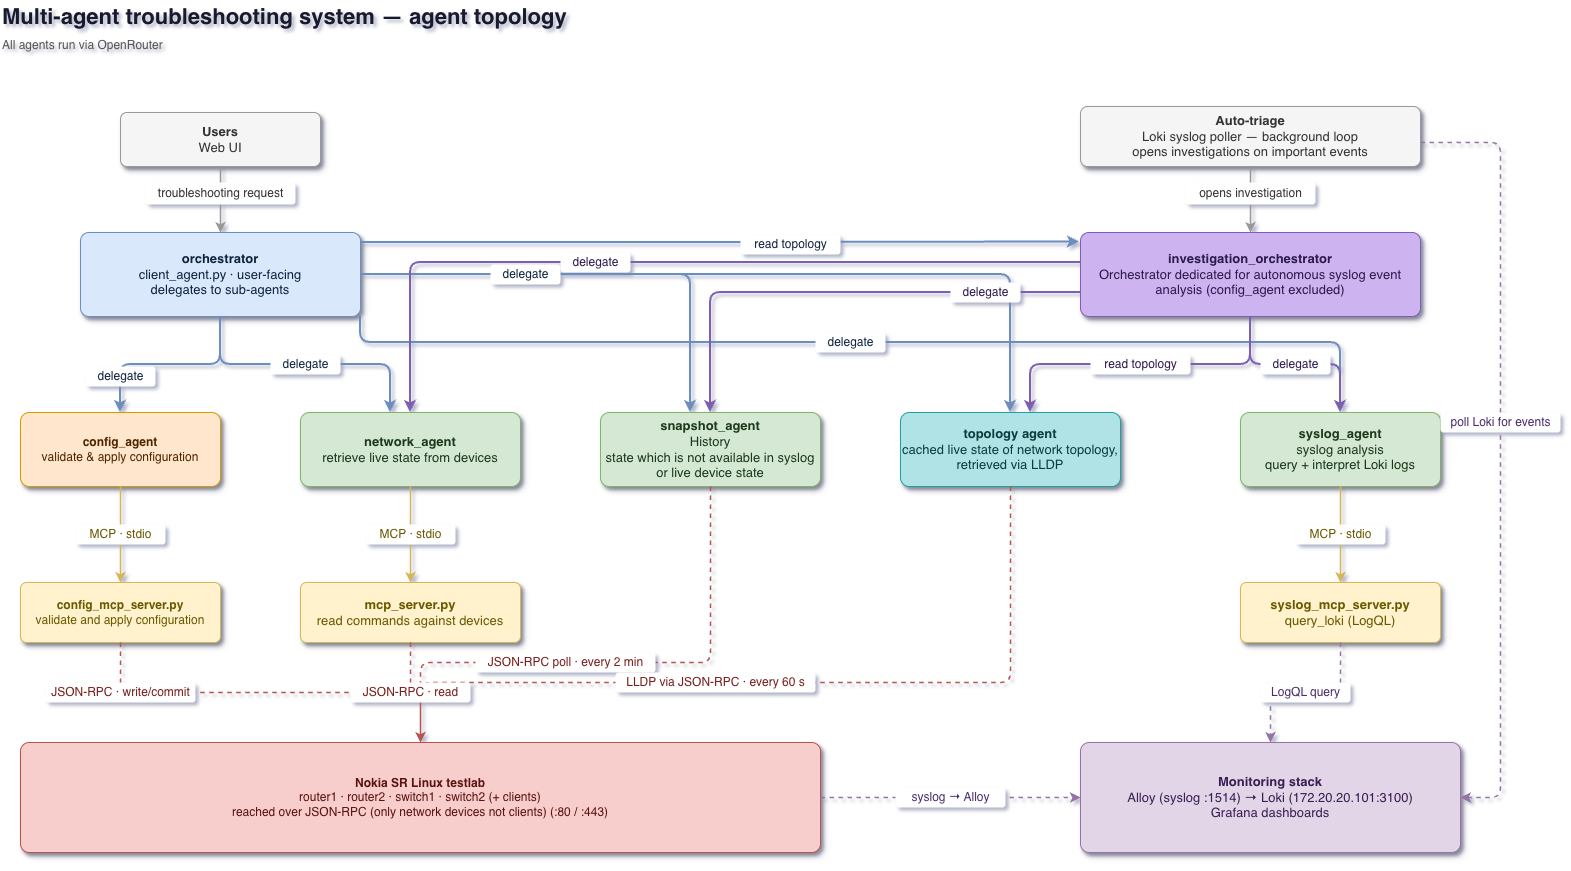
\includegraphics[width=0.9\linewidth]{graphics/agents-architecture.png}
\end{center}
\caption{Architecture of the multi-agent troubleshooting system.}
\label{fig:architecture-overview}
\end{figure}

\subsection{Agent Roles and Responsibilities}
\label{sec:agent-roles}
Each agent has a single, defined responsibility and a deliberately limited scope. The following roles make
up the system:

\begin{itemize}
    \item \textbf{Orchestrator (user-facing).} Coordinates an interactive troubleshooting session, splits
          the user's goal and delegates sub-tasks to sub-agents and synthesises their findings into a final answer. Since the sub-agents are "stateless" the orchestrator
          needs to supply all the required information to the sub-agents.
    \item \textbf{Investigation orchestrator (autonomous).} Coordiantes the autonomous syslog event based investigations. 
          It runs the same delegation pattern as the user-facing
          orchestrator without access to the config agent.
    \item \textbf{Network agent.} Retrieves live device state through read commands.
    \item \textbf{State-snapshot agent.} Provides historical device state. The state-snapshot agent focuses on information which can't be retrieved via syslog or
          device life state but can be useful for troubleshooting (like past ARP entries or routing tables).
    \item \textbf{Topology agent.} Supplies the (cached) network topology so other agents can reason about how
          devices are connected. It compares the "should be" state of the topology with the actual "live" state of the network (via LLDP queries).
    \item \textbf{Syslog agent.} Queries and analyses syslog data for the entire network.
    \item \textbf{Configuration agent.} The only agent with \emph{write} access. It is able to apply
          configuration changes to devices.
\end{itemize}

\subsection{Tool and Capability Layer}
\label{sec:tool-layer}
Agents gain the ability to interact with the outside environment through the function-calling mechanism described in
\cref{sec:func-calling}, exposed via the Model Context Protocol introduced in \cref{sec:mcp}. Rather than
exposing a single, large toolset to every agent, each agent is served by its own MCP server. This means that every agent only gets the tools
that are required for the specific task of the agent. 

This split up of expertise is a deliberate design choice that reinforces the architecture of
\cref{sec:architecture}. It keeps every agent's tool definitions, and therefore its context small and precise.

\subsection{LLM-Tier Concept}
\label{sec:model-tier-concept}
LLMs can be compared to each other using a variaty of metrics. For this work we decided to use the \emph{price per million tokens} as a comparison metric (because cost is a primary reserach question of this work).
Models are grouped into \emph{tiers} according to their \emph{price} (low, mid and high). The system is
designed so that the model tier can be varied independently of the agent logic, which makes it possible to
study how model choice affects the success rate and cost in terms of troubleshooting networking issues.
The concrete models assigned to each tier are described in \cref{sec:methodology}.

\subsection{Evaluation Concept}
\label{sec:evaluation-concept}
To answer which problem difficulties can be troubleshooted and at what success rate, the system is evaluated
against a catalogue of reproducible fault \emph{scenarios}. Each scenario injects a specific, known fault into
the network (for example a downed interface, a missing VLAN on a trunk, or a silently dropping ACL) and is
assigned a \emph{difficulty level}. The difficulty level conceptually captures how much correlation across
domains (topology, live state, history, syslog) and how many steps are required to localise the
fault.

\subsection{Use Case: Automatic Syslog Investigation}
\label{sec:autonomous-syslog-usecase}
As outlined in \cref{sec:concepts-scope}, this use case is a separate, exploratory part of the project. Its
purpose is not to be measured against the research questions but to establish \emph{whether} an autonomous,
event-driven investigation is feasible at all and how it can be integrated into the network operator's workflow. It
builds on the autonomous investigation orchestrator introduced in \cref{sec:agent-roles}. 

\paragraph{Autonomous reaction to syslog events.}
The first question is whether the system can react to the network on its own. Instead of waiting for a human
to describe a symptom, the system observes the incoming syslog stream and, when a message matching a
configured pattern arrives, automatically launches an investigation. The autonomous investigation
orchestrator then runs the same delegation pattern as the user-facing orchestrator with the execption of not having access to the configuration agent.
It is also designed so investigations cannot be opened recursively. The result is a self-contained initial report produced from a syslog event without any human
involvement.

\paragraph{Handover without duplicating work.}
The second question concerns what happens \emph{after} an autonomous investigation has run. An autonomous
report, may be incomplete or require a corrective configuration change that only a
human may authorise. The operator must therefore be able to take over and continue troubleshooting from the
point the autonomous investigation reached, without re-running the same operational commands or
re-deriving findings that have already been established. The concept addresses this by treating the
autonomous investigation's findings as reusable context (with a unique ID) that is handed to the user-facing orchestrator when
the operator resumes the case, so that the interactive session continues from the existing state rather than
starting from scratch. How this hand-over is realised concretely is described in \cref{sec:implementation}.
\section{Implementation}
\label{sec:implementation}
This section describes how the design of \cref{sec:concepts} is realised in code. It concentrates on the
decisions that shaped the implementation rather than on the code itself; the full source is available in the
project repository\footnote{\url{https://github.com/FHNW-Security-Lab-Student-Projects/ip6-autonome-netzwerkadministration}}.

\subsection{Agent Framework and Harness}
\label{sec:impl-framework}
The agent harness introduced conceptually in \cref{sec:agent-loop} is provided in this work by
\emph{Pydantic AI}, a Python agent framework \parencite{pydantic_ai}. Pydantic AI implements the agent loop,
drives the function-calling exchange with the model, manages the message history across iterations and
exposes the tools of each agent.

Every agent of \cref{sec:agent-roles} is one Pydantic AI agent, defined by four things: a name, an
instruction text (its system prompt), a model and a set of tools. The entire multi-agent system runs in a
single Python process. Agents are plain objects that call each other directly, there is no network protocol
or separate service per agent. This keeps the system simple to start, debug and reason about, an earlier
design based on an inter-agent network protocol was dropped for exactly this reason.

\subsection{Model Access}
\label{sec:impl-models}
All models are accessed through \emph{OpenRouter}, a gateway that exposes models from different vendors
behind one API \parencite{openrouter}. Switching the model an agent uses therefore only means changing a
model identifier, no vendor-specific code is involved. This is what makes the experiment matrix of
\cref{sec:experiment-matrix} practical: the same system can be swept across six models from three price
tiers without touching the agent logic.

The selected model is a runtime parameter. The orchestrator passes the active model down into every
sub-agent run, so a whole troubleshooting session runs on one model, which is required to attribute an
outcome to a single tier (\cref{sec:model-tier-concept}).

Two settings are applied centrally to every agent. First, the reasoning effort is fixed to the same level
for all models, so that model-versus-model comparisons are not distorted by each provider picking its own
default reasoning depth. Second, usage accounting is enabled on every request, so each model response
carries its native token counts. These counts are the basis for the cost and token metrics of
\cref{sec:metrics}.

\subsection{Delegation as Tool Calls}
\label{sec:impl-delegation}
Delegation between the orchestrator and its sub-agents (\cref{sec:architecture}) is realised as ordinary
function calling: each sub-agent is registered on the orchestrator as a tool. The tool description tells
the orchestrator's model what the sub-agent can do and when to use it. When the model calls the tool, the
wrapper runs the sub-agent's own agent loop to completion and returns its final answer as the tool result.

Sub-agents are stateless: they never see the orchestrator's conversation and keep no memory between calls.
The orchestrator's instructions therefore require every delegated request to be self-contained, carrying
the user's goal, the relevant details and any findings from earlier sub-agent calls. Read-only sub-agents
may be called in parallel when a request involves independent lookups.

One agent role is deliberately not backed by an LLM. The topology agent is implemented as a background task
that queries the LLDP neighbours of every device once a minute, compares them against the intended topology
definition of the lab and caches the result. The orchestrator's topology tool simply returns this cache.
Since topology retrieval is deterministic, a model in this path would add cost and latency without adding
any capability.

\subsection{Tool Servers and Device Access}
\label{sec:impl-tools}
Following the design of \cref{sec:tool-layer}, each tool-using agent is served by its own MCP server
(\cref{sec:mcp}), implemented with \emph{FastMCP} \parencite{fastmcp} and started as a subprocess of the
main process. Tool names are prefixed per domain, so tools of different agents cannot be confused.

All interaction with the lab devices goes through the JSON-RPC interface of Nokia SR Linux
\parencite{srlinux_jsonrpc}, wrapped in a single shared client module. The tools offer two routes to device
data: executing formatted \texttt{show} commands, and reading a specific YANG path directly from the state
or running-configuration datastore. The agent instructions explain when each route is appropriate. To keep
the models from inventing plausible-looking but invalid commands, a reference of valid SR Linux read
commands is embedded in the network agent's system prompt. When a device still rejects a command, the
failure is detected in the tool output and recorded, this is the source of the invalid-command count of
\cref{sec:metrics}.

For syslog, all devices log to a central \emph{Loki} instance \parencite{grafana_loki}, which the syslog
agent queries through its MCP tool. A practical problem here is time: an LLM has no reliable clock and its
prompt may be minutes old by the time a tool runs. The tools therefore accept time expressions such as
\enquote{now}, a relative offset (\enquote{15m ago}) or an absolute timestamp, and resolve them against the
real clock at call time. The model only ever states its intent and never computes timestamps itself.

\subsection{Context Management}
\label{sec:impl-context}
Device output is the dominant source of token growth: every iteration of an agent loop re-sends the full
message history, so large tool returns are paid for again on every subsequent step. Observed runs of the
network agent reached several hundred thousand input tokens for a single query before countermeasures were
in place. Two measures address this, both following from \cref{sec:tokens-context-cost}.

The first works at the source. Tool responses are serialised compactly and cut off at a fixed size; a
truncated response ends with a note telling the model to re-query a narrower path instead. The instructions
additionally steer the model towards narrow queries (a single leaf across all interfaces rather than the
whole interface tree).

The second works on the history. Before each model request, a processor estimates the current prompt size,
anchored on the token count the provider reported for the previous request. Only when the estimate
approaches the model's context window (whose size is looked up per model, since the swept models differ
considerably) does it act: the oldest oversized tool returns are replaced by a one-line stub stating which
tool was called and that it can be re-invoked if the output is needed again. The most recent returns and
all error messages are always kept verbatim, errors carry the correction the model needs to avoid repeating
a bad call. This keeps long runs inside the context window, reduces cost and counters the
\enquote{lost in the middle} degradation without hiding any information the model cannot get back.

\subsection{Guarding Configuration Changes}
\label{sec:impl-config}
The configuration agent is the only write path into the network, and its use is guarded by a two-step
workflow encoded in the orchestrator's instructions. A change request is first delegated as
validation-only: the agent loads the commands into the device's candidate configuration and returns the
resulting diff without committing. The orchestrator shows this diff to the user, and only after explicit
approval does it send the apply request, which must carry the exact commands from the validation step. A
request without a clear prefix is treated as validation, so the default is always the safe path. The
autonomous investigation orchestrator has no access to the configuration agent at all
(\cref{sec:agent-roles}).

\subsection{Autonomous Investigations and Handover}
\label{sec:impl-investigations}
The syslog use case of \cref{sec:autonomous-syslog-usecase} is driven by a background task that polls Loki
every 30 seconds for messages of severity error and above. A matching event opens an investigation, keyed
by device and message so that a repeating log line does not spawn duplicates, and starts a triage run of
the investigation orchestrator in the background. Because this orchestrator lacks the tools to open or
continue investigations, an investigation can never trigger further investigations recursively.

Each investigation is persisted to disk as a record containing an identifier, the affected device, the
triggering log line and its timestamp, the current status, a summary, and, crucially, the complete
serialised message history of the agent run. This history is what realises the handover described in
\cref{sec:autonomous-syslog-usecase}: the user-facing orchestrator has tools to list, inspect and continue
investigations, and continuing a case loads the stored history and resumes the investigation orchestrator
on top of it. The model therefore still holds all earlier findings and tool results and continues from
where the autonomous run stopped, instead of re-running the same commands.

\subsection{Interfaces and Instrumentation}
\label{sec:impl-interfaces}
The system has three entry points: a terminal chat for development, a web chat interface with a model
selector (built on the framework's bundled web UI), and a status page showing all open investigations. In
the interactive interfaces the orchestrator keeps its message history across turns, so a troubleshooting
session is one continuous conversation.

All agent runs, tool calls and device requests are traced with \emph{Logfire} \parencite{logfire}. The
traces show, per run, which sub-agents were called with which requests and what each tool returned, which
was the main debugging instrument during development and was also used to verify the recorded token and
cost figures.

The experiments of \cref{sec:methodology} reuse the interactive system unchanged, except that the
configuration agent and the investigation tools are disabled through feature flags, so the measured system
is exactly the read-only troubleshooting core. The delegation wrappers record the usage of every sub-agent
run into the experiment log, from which the metrics of \cref{sec:metrics} are derived.

\section{Methodology}
\label{sec:methodology}

% TODO: Experiment setup — test environment, scenarios and difficulty levels.

\section{Evaluation}
\label{sec:evaluation}

% TODO: Discussion — time saved, cost saved, and success rate per difficulty level.

\section{Conclusion and Future Work}
\label{sec:conclusion}

% TODO: Summarize the findings and outline potential future work.


%%---AUXILIARY TOOLS---------------------------------------------------------------------
\section{Auxiliary Tools}
\label{sec:auxiliary_tools}

The following tools were used in the creation of this work:

\begin{itemize}
    \item \textbf{DeepL write} -- To rephrase
    \item \textbf{Claude Code / Claude AI} -- Programming / templating / grammer and spelling mistakes
    \item \textbf{Google Scholar and Google Scholar Labs} -- For research
    \item \textbf{Consensus AI Research} -- For research
\end{itemize}

%%---BIBLIOGRAPHY------------------------------------------------------------------------
{\sloppypar
\printbibliography[heading=bibintoc, title=References]
}

%%---APPENDIX----------------------------------------------------------------------------
\selectlanguage{english}				%ngerman or english
\include{sections/authenticity}
\selectlanguage{english}				%ngerman or english
% Top-align figures that land alone on a float page (default vertically centers them)
\makeatletter
\setlength{\@fptop}{0pt}
\makeatother

\begin{appendix} %Anhang
\section{Appendix}
\label{sec:appendix}

\subsection{Model Prices During the Experiment Window}
\label{app:model-prices}

The per-run costs in the experiment log are computed as native token counts times the model's
advertised OpenRouter price at run time. \Cref{tab:recovered-rates} lists the rates in effect.
Only GLM-5.2 changed price during the window. The open-weight models (GLM-5.2, DeepSeek-V3.2,
Ministral-14B) are served by multiple competing providers on OpenRouter, so their advertised
price is whatever the cheapest provider currently charges and can move at any time.

\begin{table}[htbp]
\centering
\small
\begin{tabular}{@{}llrr@{}}
\toprule
\textbf{Model} & \textbf{Period} & \textbf{Input \$/Mtok} & \textbf{Output \$/Mtok} \\
\midrule
anthropic/claude-opus-4.8    & whole window          & 5.00   & 25.00 \\
openai/gpt-5.5               & whole window          & 5.00   & 30.00 \\
qwen/qwen3.7-max             & whole window          & 1.25   & 3.75  \\
deepseek/deepseek-v3.2       & whole window          & 0.2288 & 0.3432 \\
mistralai/ministral-14b-2512 & whole window          & 0.20   & 0.20  \\
z-ai/glm-5.2                 & 2026-06-29            & 0.95   & 3.00  \\
z-ai/glm-5.2                 & 2026-06-30            & 0.94   & 3.00  \\
z-ai/glm-5.2                 & 2026-07-02 -- 07-03   & 0.93   & 3.00  \\
\bottomrule
\end{tabular}
\caption{OpenRouter list prices per million tokens during the experiment window.}
\label{tab:recovered-rates}
\end{table}

\subsection{Additional Experiment Figures}
\label{app:extra-figures}

\Cref{fig:invalid-commands} shows the malformed device commands as totals over the five runs of
each scenario--model pair. \Cref{fig:scenario-ttd} breaks the time to a correct diagnosis down
to scenario level (correct, completed runs only). A missing row means the model never solved
that scenario. \Cref{fig:wall-clock-distribution} shows the wall-clock time of all 300 runs,
including wrong diagnoses and DNFs. The runs stopped by the time limit form the clusters at
the 600-second cap.

\begin{figure}[htbp]
\begin{center}
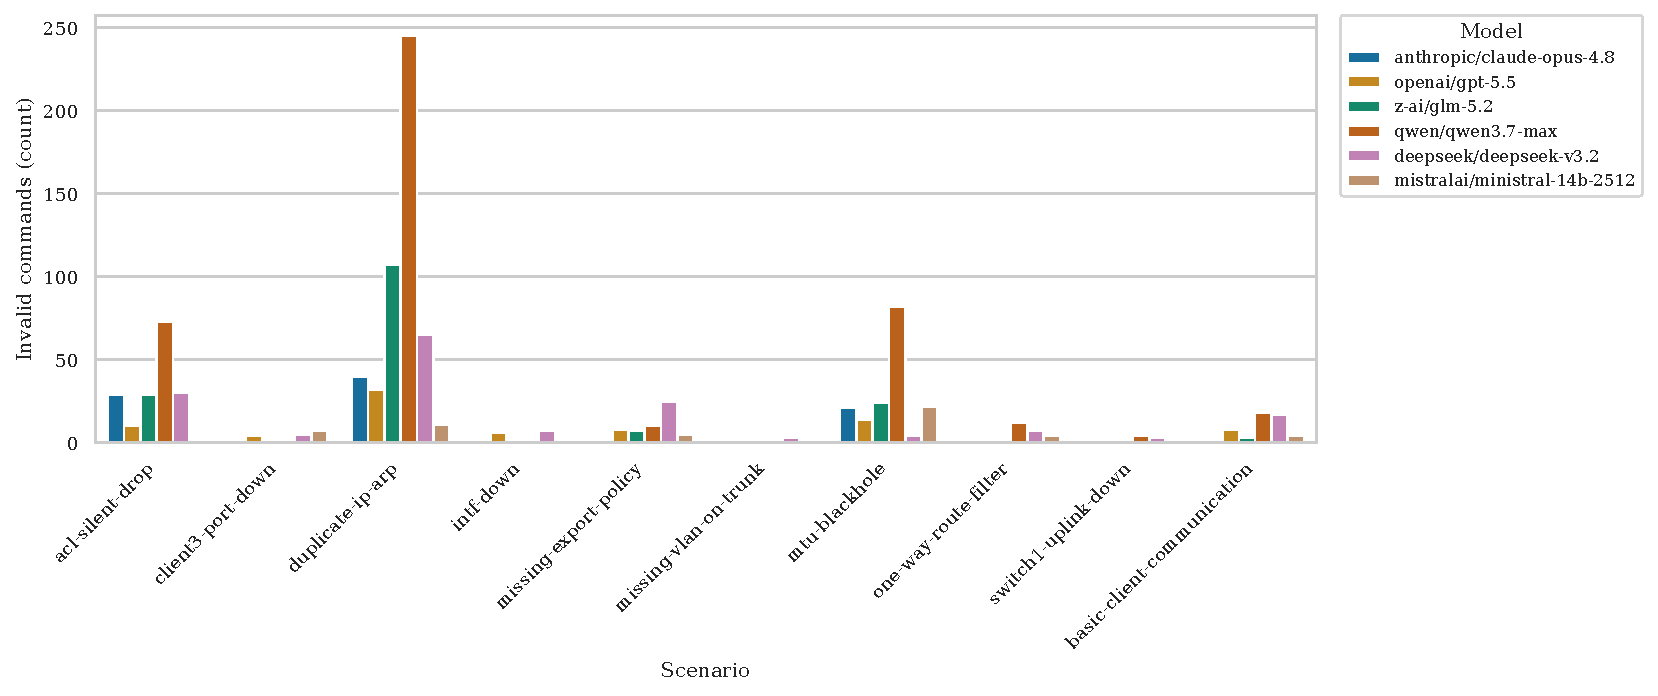
\includegraphics[width=\linewidth]{graphics/invalid_commands.pdf}
\end{center}
\caption{Malformed device commands per scenario and model.}
\label{fig:invalid-commands}
\end{figure}

\begin{figure}[htbp]
\begin{center}
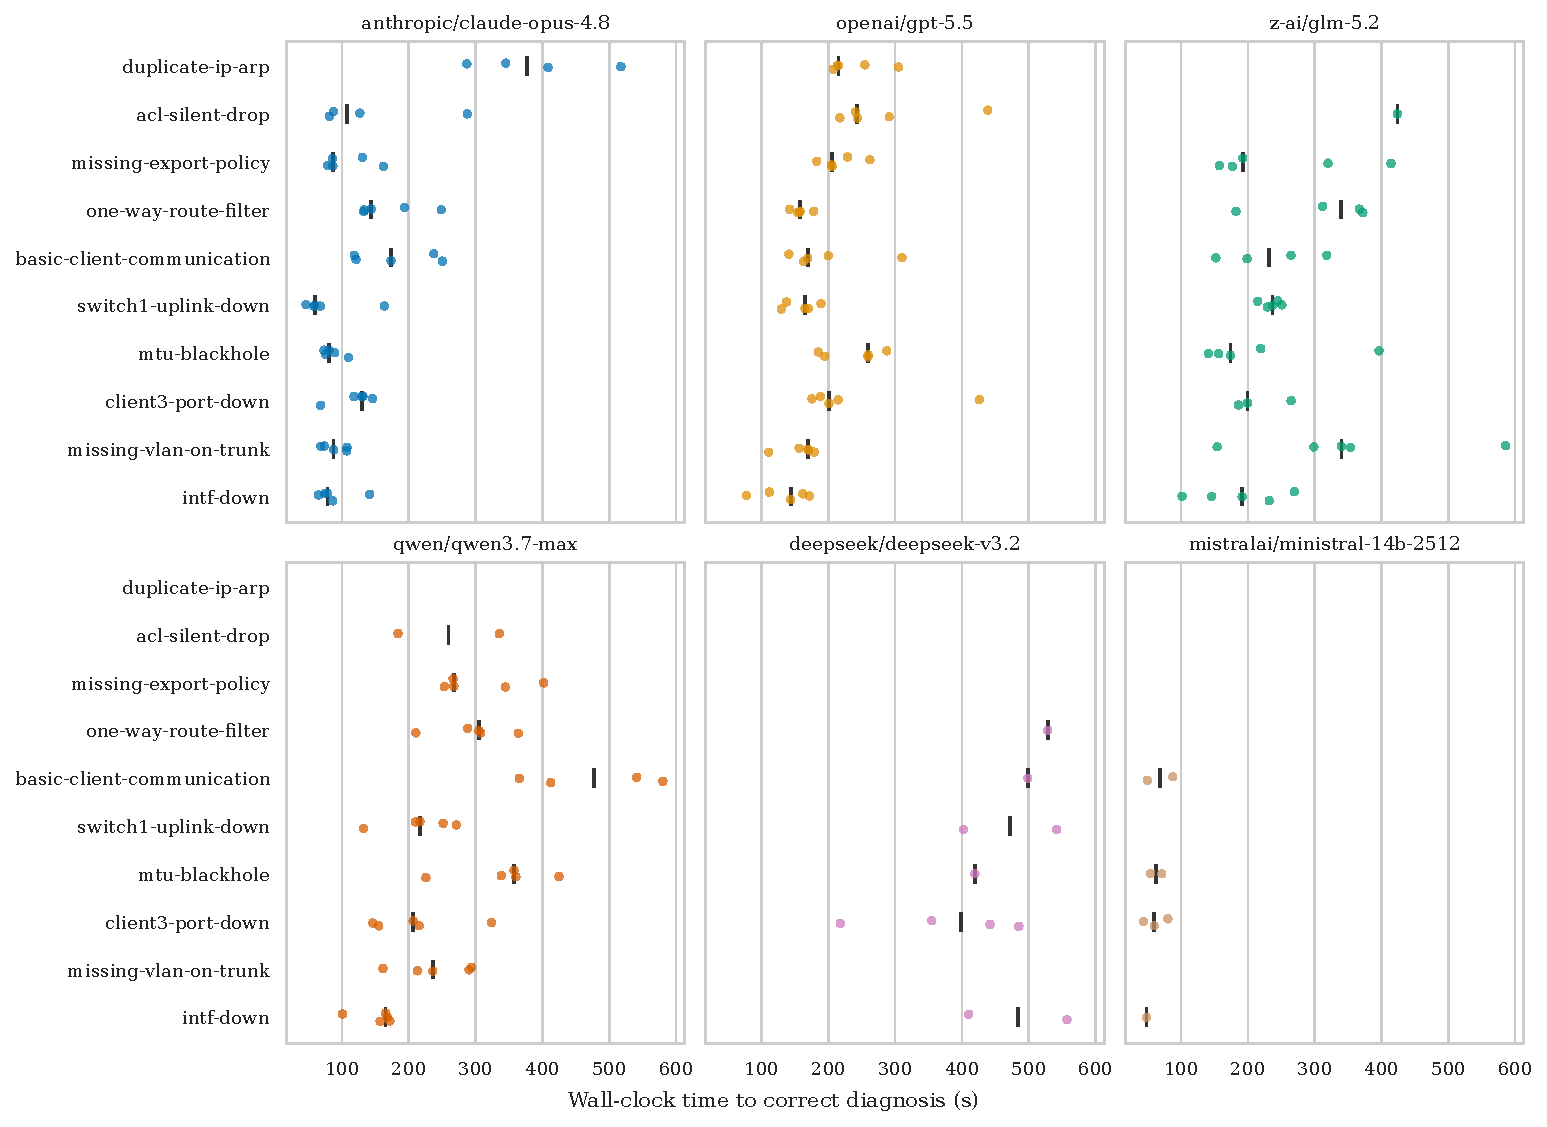
\includegraphics[width=0.8\linewidth]{graphics/scenario_time_to_diagnosis.pdf}
\end{center}
\caption{Wall-clock time to a correct diagnosis per scenario and model.}
\label{fig:scenario-ttd}
\end{figure}

\begin{figure}[htbp]
\begin{center}
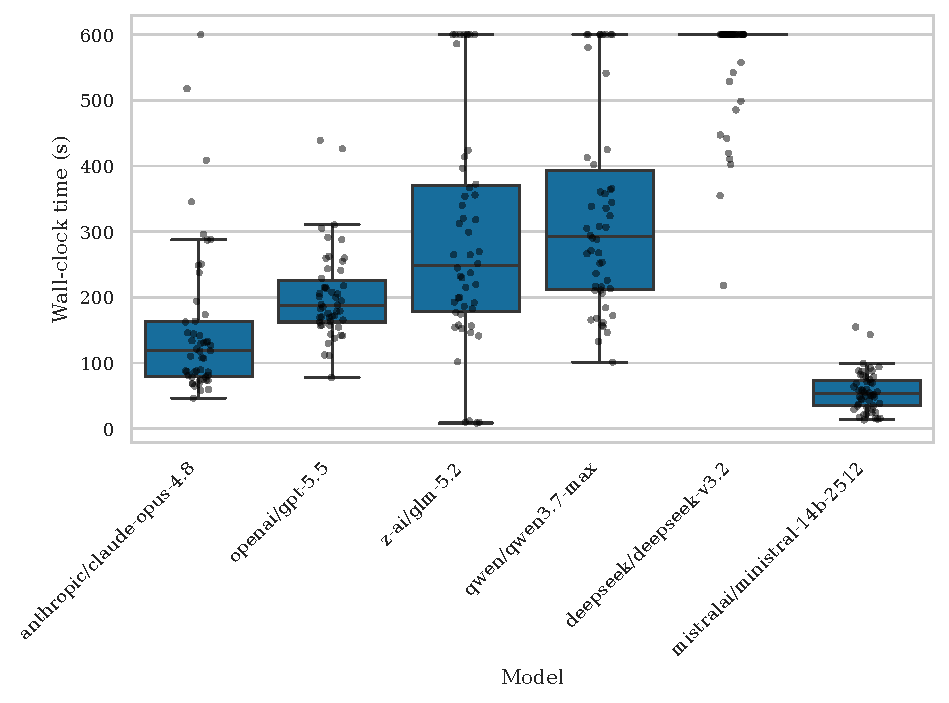
\includegraphics[width=0.85\linewidth]{graphics/distribution_wall_clock.pdf}
\end{center}
\caption{Wall-clock time per run over all 300 runs, including wrong diagnoses and DNFs.
Boxes show median and interquartile range. Dots are individual runs. The clusters at 600\,s
are the 55 runs stopped at the wall-clock cap.}
\label{fig:wall-clock-distribution}
\end{figure}

\clearpage
\subsection{User Interface Screenshots}
\label{app:ui-screenshots}

\Cref{fig:chat-interface} shows the web chat interface of \Cref{sec:impl-interfaces} in a troubleshooting scenario (a conversation).
\Cref{fig:investigation-status} shows the status page of the
autonomous syslog investigations (\Cref{sec:impl-investigations}). Each row is one automatically
opened case with its device, state and a summary of the findings. The detail view below lists the
triggering syslog event and the stored report of the selected case.

\begin{figure}[htbp]
\begin{center}
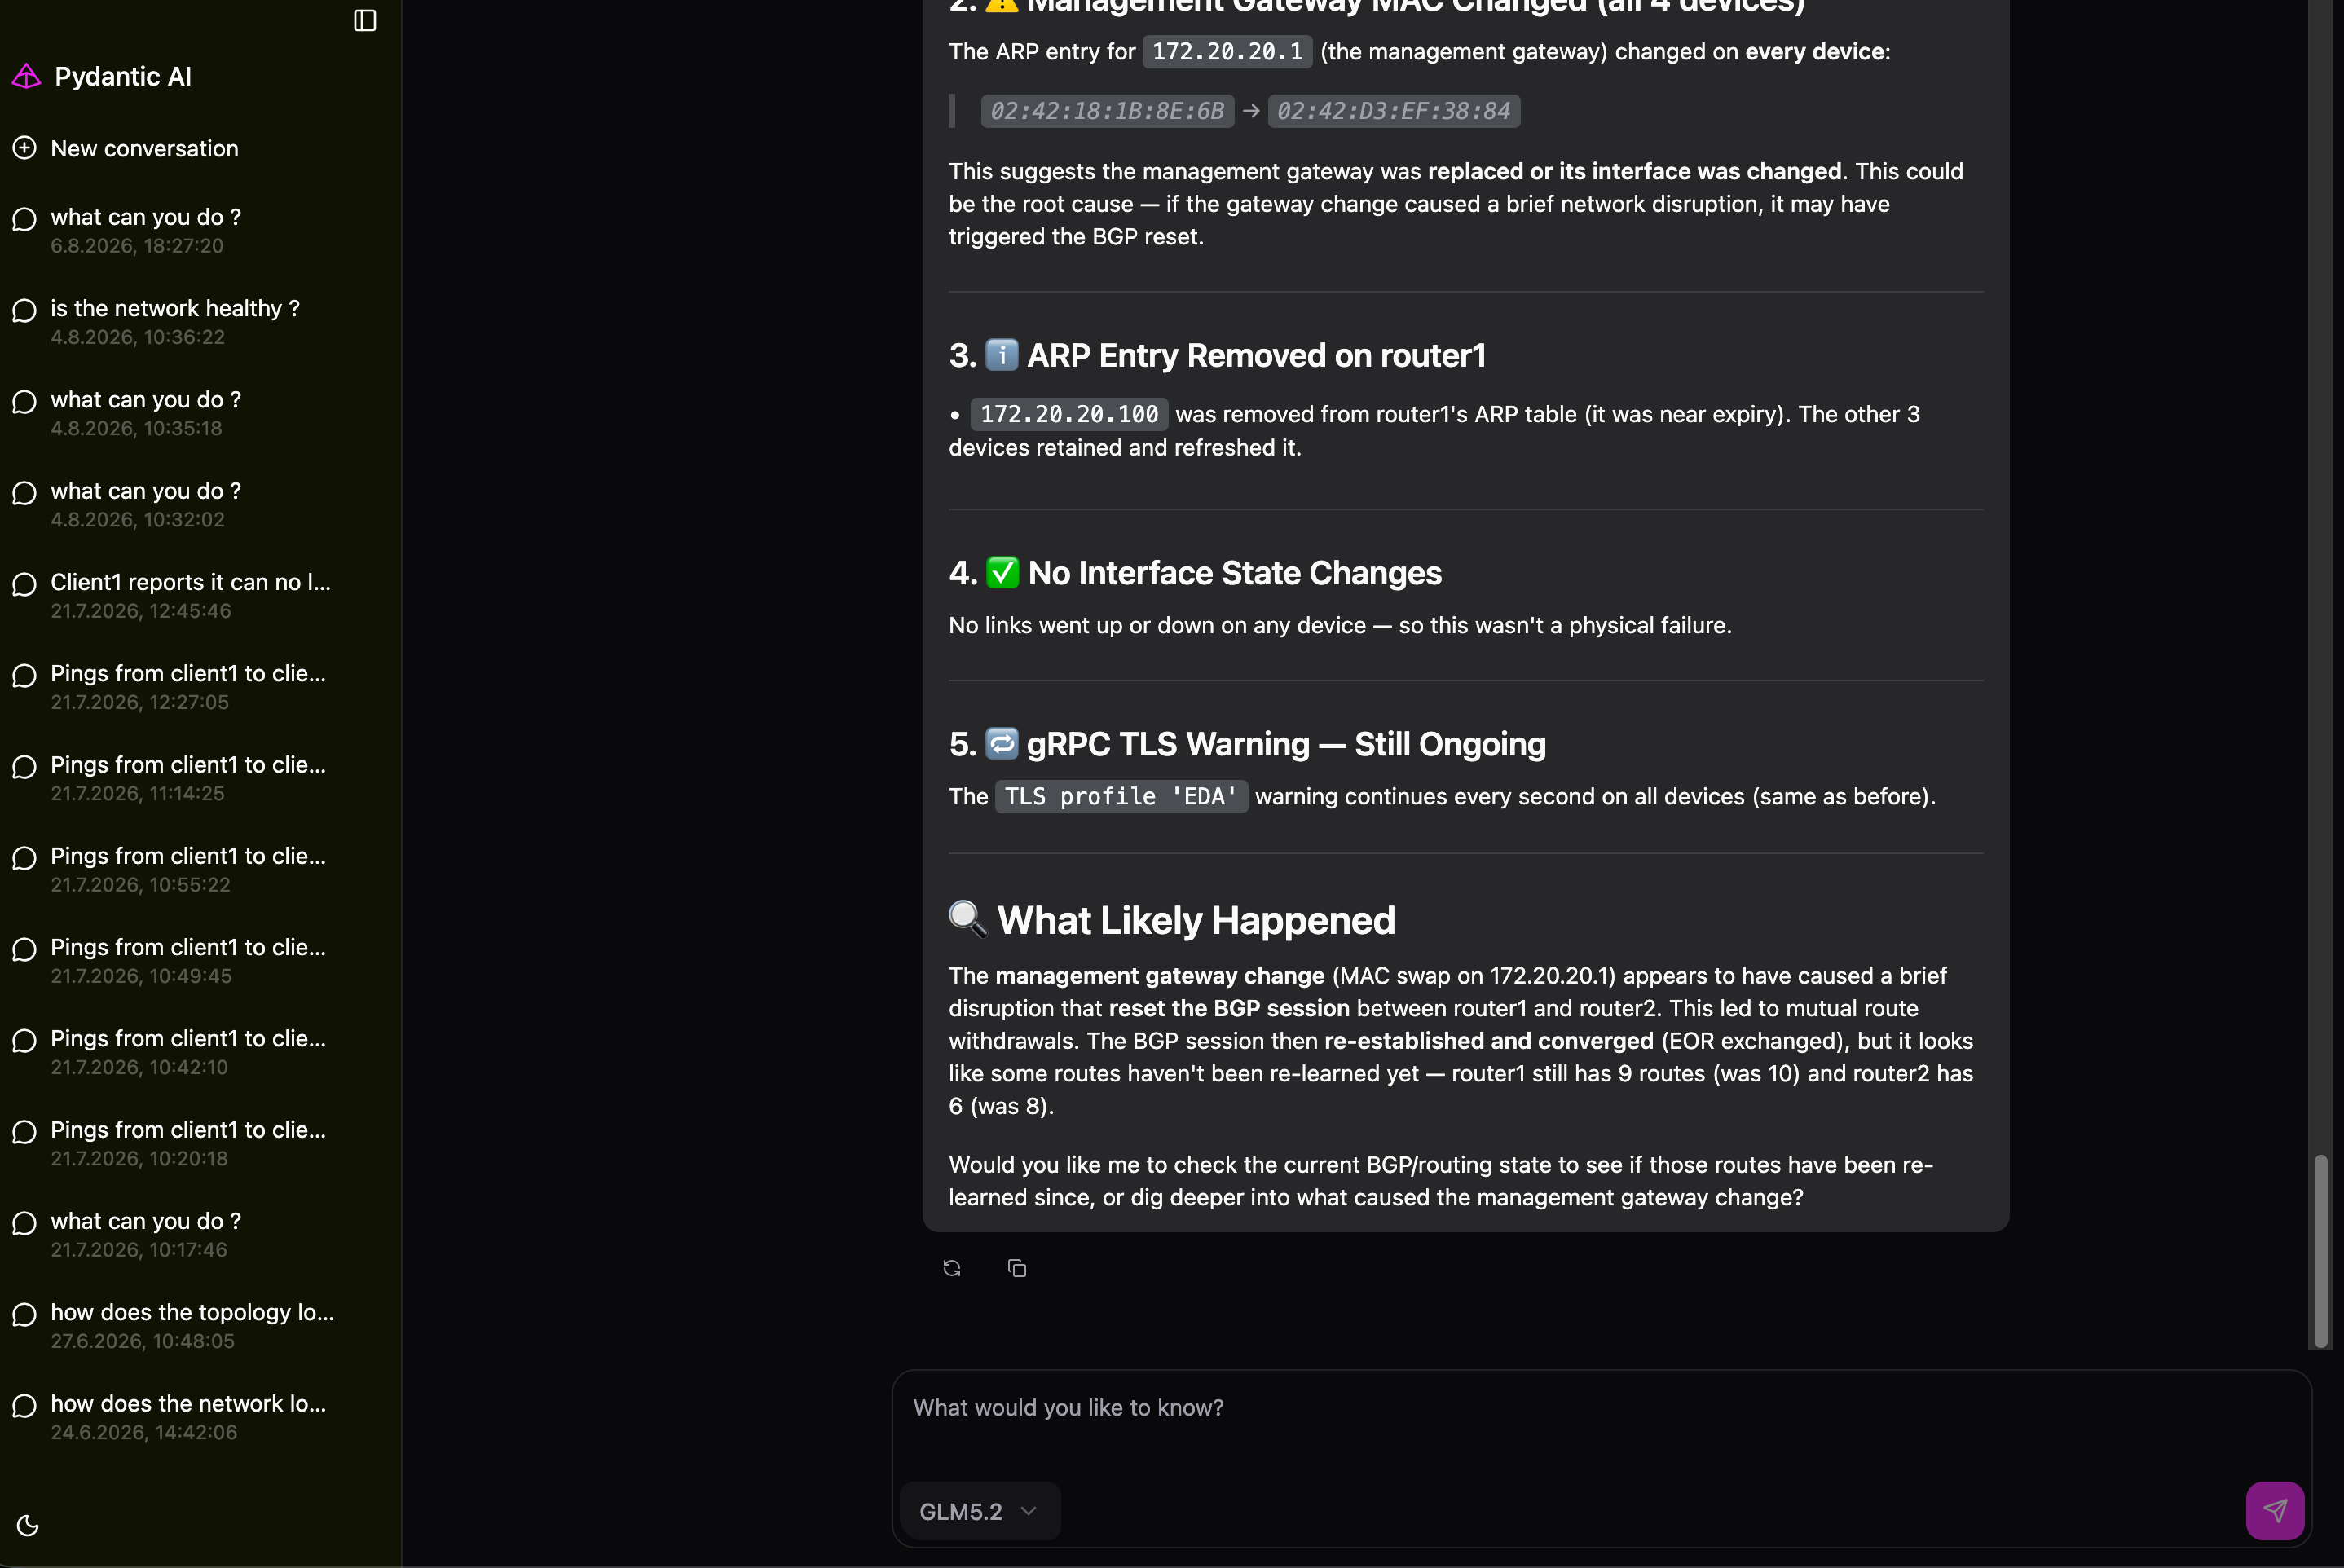
\includegraphics[width=\linewidth]{graphics/chat-interface.png}
\end{center}
\caption{The web chat interface with model selector, showing the closing answer of a
troubleshooting conversation.}
\label{fig:chat-interface}
\end{figure}

\begin{figure}[htbp]
\begin{center}
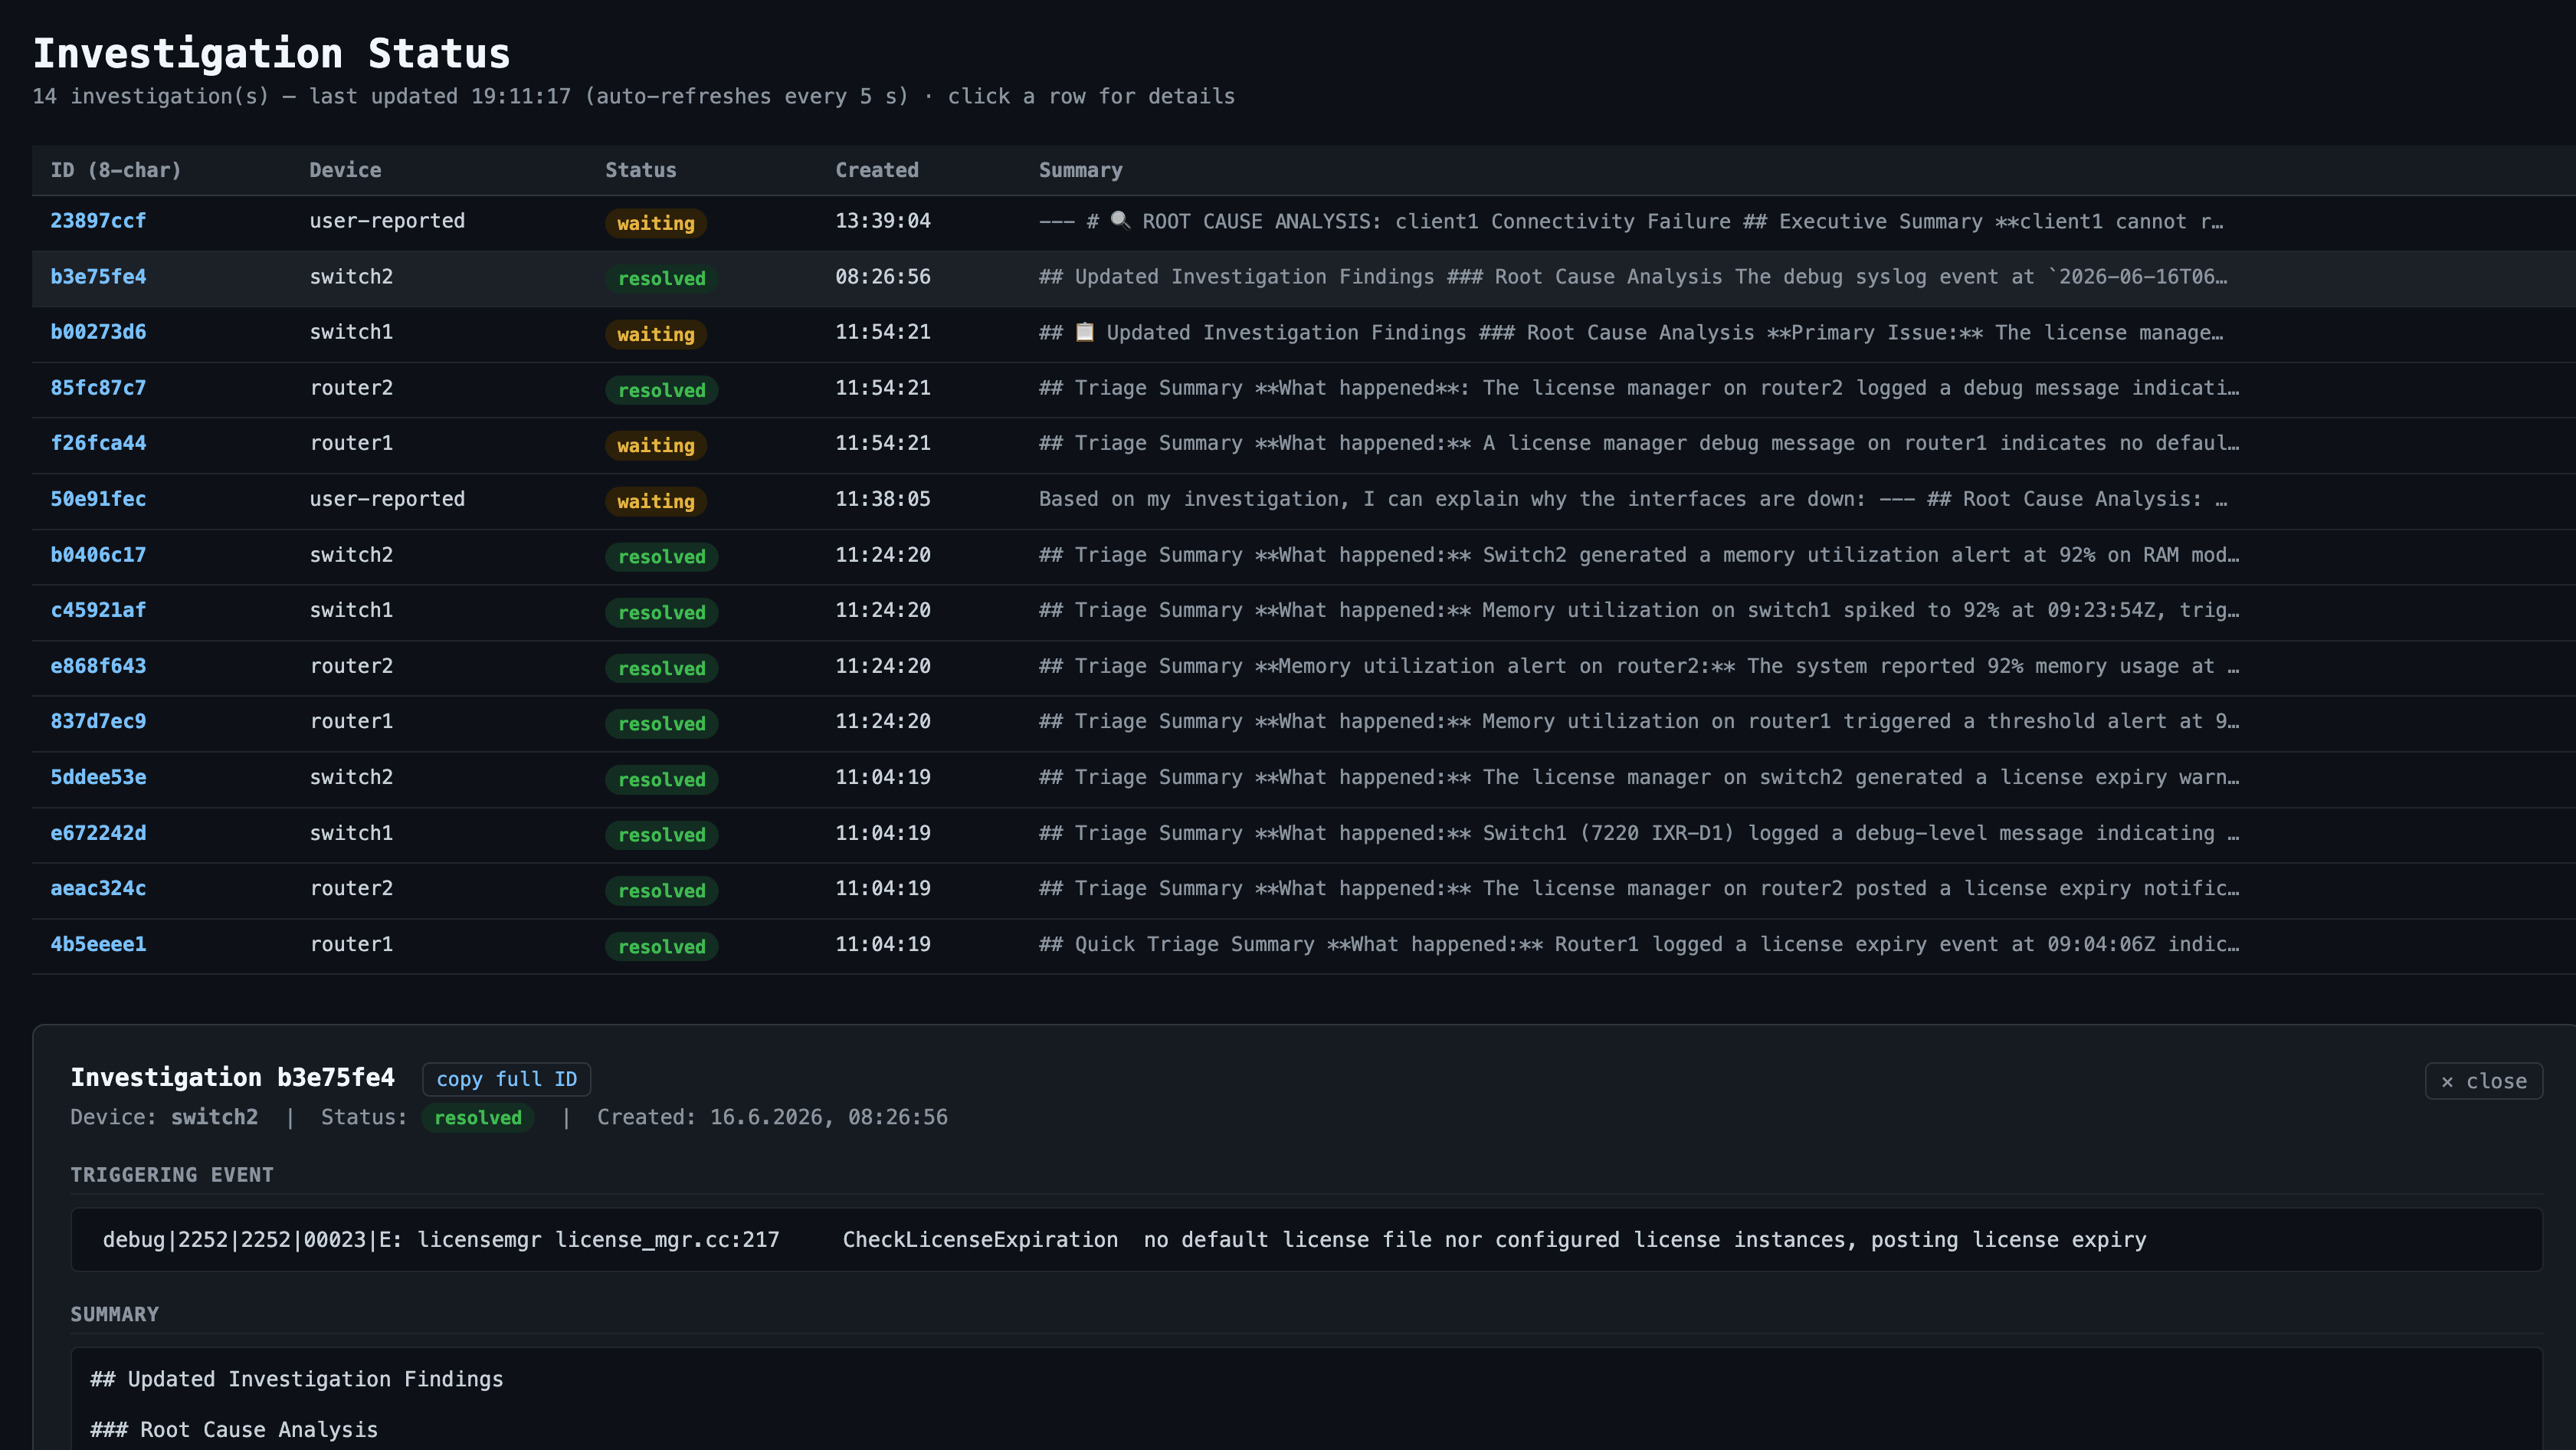
\includegraphics[width=\linewidth]{graphics/automatic-investigations.png}
\end{center}
\caption{The status page of the autonomous syslog investigations, with the list of open and
resolved cases and the detail view of one resolved investigation.}
\label{fig:investigation-status}
\end{figure}

\end{appendix}


%%---NOTES for DEBUG---------------------------------------------------------------------
%\newpage
%\listoftodos[\section{Todo-Notes}]
%\clearpage

\end{document}
